
%\clearpage
\section{Definitions and Notation}
\label{sec:tm}

In this section, a formal approach to networks and traffic matrices is
defined.  Traffic originates from a \emph{source} and is delivered to
a \emph{destination} (or several destinations). The traffic traverses
a set of \emph{links} between some set of sources and destinations.
The links connecting these define the \emph{topology} of the network,
and the paths chosen by traffic flows determine the {\em
  routing}. Traffic may be split across multiple paths by load
balancing, or may keep to a single path.  Often, sources and
destinations are identified with network devices such as switches or
routers, but they can also refer to a location in a logical space
attached to the network, for instance IP addresses of prefix blocks.

Let $\Omega$ denote the non-empty set of all sources and destinations
in a network and let $|\Omega| = N$.  The sources and destinations
often have a physical, geographic location, and so we regard their
indices as {\em spatial variables}, even when they are actually
logical entities, such as Autonomous Systems (ASes), or cannot be
directly identified as network devices, as with IP addresses.

\begin{figure}
  \begin{center}
    \begin{minipage}[m]{0.64\columnwidth}
      \vspace{0pt}
      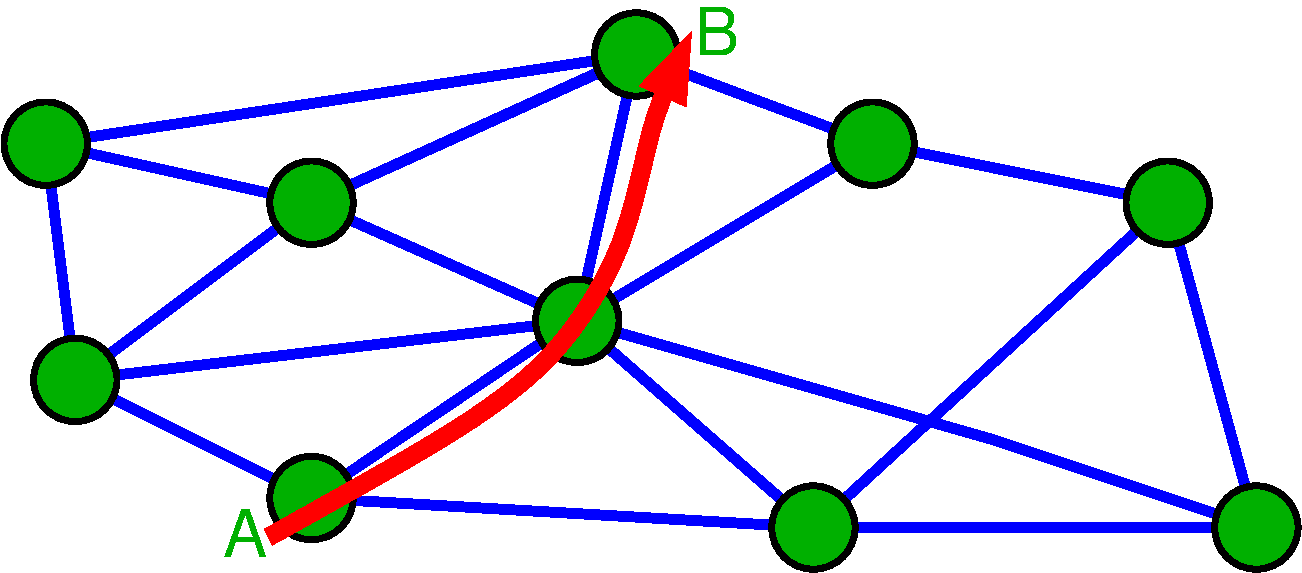
\includegraphics[width=0.9\columnwidth]{traffic_matrices.pdf}      
    \end{minipage}
    \hspace{-10mm}
    \begin{minipage}[m]{0.3\columnwidth}
      \vspace{0pt}
      $$ X = \displaystyle
              \left( \begin{array}{lllll}
                x_{AA} & {\color{red} x_{AB}} & x_{AC} & \cdots \\
                x_{BA} & x_{BB} & x_{BC} & \cdots \\
                \vdots & \vdots & \vdots & \ddots \\
	      \end{array} \right)
    $$
  \end{minipage}
  \caption{An example of a traffic matrix. Note that often the
    diagonal elements, $x_{AA}, x_{BB}, \ldots$ are zero as this
    traffic does not cross the network, however, in almost as many
    cases it is non-zero because a ``node'' in the graph represents an
    aggregation of devices such as a PoP or an AS. In these cases we
    often do wish to measure these diagonals, even though they may not
    cross the logical links pictured, because they affect traffic
    engineering within the PoP, for example.
  \label{fig:tm} }
  \end{center}
\end{figure}


A traffic matrix is naturally represented by a three dimensional,
nonnegative hyper-matrix $\bX(t)$, with $i,j$-th entry $X_{i,j}(t)$.
Each entry represents the traffic volume, or demand, measured in terms
of bytes or packets, from source $i$ to destination $j$ in time
interval $\lbrack t, t+\Delta t) \subset \cT$, the full measurement
interval being denoted by $\cT$. As an aside, a matrix representation is
useful for the representation of other aspects of the network, for
instance, delay, jitter, loss, bottleneck-bandwidth and distance
\cite{Medina02Taxonomy}, but throughout the chapter, traffic will be
the focus. Whenever the context is clear, for example, when
considering only the spatial structure of the matrix, the time index
$t$ is dropped. An abstract example of the traffic matrix is presented
in \autoref{fig:tm}.

A closely related concept is the {\em demand matrix}, distinct from
the traffic matrix because the former is {\em offered load}, and the
latter {\em carried load} \cite{Feldmann01TMdemand}. 
They may be the same, but may differ where
congestion limits the carried traffic, or rate limiting is used on
some traffic streams. In general we cannot measure offered traffic,
only carried traffic, and so almost all empirical research has
concentrated on traffic matrices, but it is important to note that
many of the assumptions of traffic matrix models are actually
motivated by intuition about demand matrices, and these may not apply
where the two differ substantially\footnote{Many works make no
  distinction between demand and traffic matrices, leading to
  confusion. Here, we shall try to keep the two distinct: when we say
  traffic matrix, we are referring to carried traffic.}.


% The spatial variable $i$ and $j$
% are generally associated with the address structure of the Internet,
% such as Internet Protocol (IP) addresses, or prefixes of these
% addresses.

Large-scale, real-time monitoring of traffic is intractable at
present, thus limiting measurements to the average traffic in a
discrete time interval. Shorter time intervals \ie~small $\Delta t$,
benefit anomaly detection applications, the tradeoff being a
possibility of uncertainty from traffic burstiness at shorter time
scales combined with larger potential measurement or sampling
errors\footnote{Traffic is typically sampled at the backbone network
  level to cope with the tremendous volumes of data that could be
  collected.}. Longer time intervals result in ``smoother'' traffic, 
  averaging out measurement errors. However, this smooths out
real variability in the traffic as well, and can result in meaningless
estimates in the presence of strong non-stationarity. Hence, the
choice of $\Delta t$ depends on the application and available
measurements. Common choices range from 5 minutes to an hour. Further
discussion on the temporal properties of traffic flows is found in
\autoref{sec:models}.

There are two popular definitions of traffic matrices: the
origin--destination (OD) matrix and the ingress--egress (IE) matrix.
\begin{enumerate}

\item \textbf{OD traffic matrix}: this matrix measures traffic from
  true source to destination, \ie~the point that generates a packet
  to the point that receives it. In the Internet, it is perhaps most
  reasonably defined in terms of Internet Protocol (IP) addresses.
  However, if $\Omega$ is defined over the entire IPv4 address space of
  $2^{32}$ addresses (with even more for IPv6), this poses storage and
  computational problems. Moreover, the matrix would be very
  sparse. What's more, protocols such as NAT, HTTP proxies and
  firewalls may obscure the true IP address mappings. One way to
  overcome some of these deficiencies is to aggregate the traffic
  matrix into blocks of IP addresses, frequently using routing
  prefixes. Bharti \etal \cite{Bharti10Invisible} defined the idea of 
  \textit{atomic aggregation}
  to partially circumvent the problem of size of an OD matrix. 
  If the logical indexing chosen is \textit{atomic}, then a 
  non-zero element of an OD traffic matrix implies that all 
  flows between the particular source and destination 
  pair is fully visible to the network operator (see \cite{Bharti10Invisible}
  for details).	

\item \textbf{IE traffic matrix}: any single network operator sees
  only a small proportion of the Internet OD matrix. Thus this matrix
  is not just unknown, but unmeasurable (by a single
  operator). Instead, many operators find that using their edge
  routers (or even the edge links) as sources and destinations results
  in a local traffic matrix of great use. We call this the IE traffic
  matrix as the set $\Omega$ includes ingress, \ie~traffic going into
  the network, and egress, \ie~traffic flowing out of the network,
  points as proxies for sources and destinations. A single ingress or
  egress ``node'' may denote a router, a collection of physically
  co-located routers called a Point of Presence (PoP), or some other
  abstract collection of traffic ingress/egress points depending on
  the level of coarseness required in the modelling process. The PoP
  level convention is often adopted as it provides a simple
  visualisation of the network its operators.
\end{enumerate}

IE traffic matrices can be obtained in a number of ways. They can be
formed from OD traffic matrices simply by mapping IP prefixes to
ingress/egress locations in the network, but this assumes knowledge of
all flows traversing the ingress/egress nodes.  Traffic at egress
nodes may be inferred from router data (see the next section) and
measurements of ingress traffic, but typically, the converse is
difficult. Likewise, it is usually difficult to form an OD matrix from
IE matrices.

Consequently, the IE traffic matrix is frequently adopted for network
optimisation applications as it is more practical to measure, and
because in aggregating traffic the OD flows are ``bundled'' together
into locally meaningful groupings. A network may carry flows between
billions of IP address pairs and millions of prefix pairs, but only
thousands of router pairs, and hundreds of PoP pairs.  In this way,
the IE matrix is a more compact representation, but more importantly,
the aggregation of the traffic into large bundles results in a
smoothing effect on the data, reducing the number of independent
parameters that may have to be estimated. At the PoP level, the
aggregation of flows results in averaging out sampling error (similar
to the choice of $\Delta t$ above). This is highly beneficial for
numerical iterative algorithms used to estimate the traffic matrices,
as aggregation leads to better conditioning of the traffic matrix. The
trade-off, unfortunately, is the loss of fine grained data, as one can
no longer observe IP-level flow data, or examine application profiles.

Another consideration worthy of concern in applying traffic matrices
is {\em invariance}.  A good representation of the traffic has
to be invariant to other network aspects, such as routing and the
network topology. For instance, if the traffic matrix for a network
changes in response to changes in link placement, then the matrix is
not terribly useful for network design. IE matrices are subject, for
example, to large changes due to routing shifts, and this means that
they are less useful to operators compared to OD matrices. However,
the practicalities of measurements mean that IE matrices may be all
that is measurable.

% That leads naturally to our next topic: measurement of traffic
% matrices. 

% Another example was discussed in \cite{Alderson06Topology} using the G\'{E}ANT \cite{GEANT} network for illustration, where a 
% regional network uses the G\'{E}ANT router to transit traffic within the regional network itself. The result is a net increase of the traffic 
% demands at the nodes being used for this purpose, although these demands themselves do not traverse G\'{E}ANT. Also, distortions 
% may occur in the form of hot potato routing \cite{Paxson97Routing}; see Section \ref{sec:models}. Despite 
% these issues, due to the practicality of the IE traffic matrix, focus will generally be on the IE traffic matrix, unless specified otherwise.



\subsection{Example}

As an example we present the Abilene (Internet2) data from 2004 that
was used in several studies
\cite{Zhang05Anomography,Roughan05GravSynth,Alderson06Topology}.  The
backbone network is located in North America (see
\autoref{fig:abilene_2004_map}).  The traffic data contains averages
over 5 minute intervals, from March 1st to September 11th, 2004
(though there are some missing periods).  The dataset is an
Ingress-Egress, router-router\footnote{In Abilene, at the time, the
  routers almost corresponded to PoPs.} traffic
matrix. \autoref{tab:traffic_matrix} shows one example traffic matrix
from that period, along with row and column sums.

% created by TrafficMatrix::latex_write
% source = Abilene/Internet 2 network
% time interval = 5 minutes
% topology = 
% time = 16-25-00
% date = 2004-04-15
% name = Abilene, 2004
% sampling = 1 in 100 packets
% additional information = as measured using netflow
% created by = TrafficMatrix::write, version 1
% type = ingress/egress, router/pop-level, traffic matrix
% cite = Network Anomography, Yin Zhang, Zihui Ge, Albert Greenberg, Matthew Roughan, ACM/Usenix Internet Measurement Conference, Berkeley, CA, USA, 2005.
% creation date = Mon Jun 24 15:21:43 CST 2013
% units = Gbytes / second
\begin{sidewaystable}[htp]
  \centering
%  \footnotesize
  \begin{tabular}[htp]{r|rrrrrrrrrrrr|r}
          & \multicolumn{12}{c|}{Destination} & \\
      Source &   1 &   2 &   3 &   4 &   5 &   6 &   7 &   8 &   9 & 10 &  11 &  12 & Row sum \\
    \hline
   1 &    0.07 &     0.07 &     0.43 &     0.00 &     0.06 &     0.12 &     0.06 &     0.00 &     0.05 &     0.00 &     0.00 &     0.25 &     1.12 \\
   2 &    0.00 &     4.09 &     6.42 &     0.06 &     7.07 &     4.42 &     1.59 &     0.02 &     3.24 &     0.03 &     0.16 &    11.09 &    38.18 \\
   3 &    0.00 &     4.70 &    25.48 &     4.11 &    13.99 &    11.53 &     3.31 &    87.27 &     5.22 &     0.01 &     0.08 &     7.70 &   163.38 \\
   4 &    0.00 &     1.93 &    10.25 &     1.68 &     5.63 &     6.11 &     2.59 &     0.01 &     4.11 &     2.60 &     0.04 &     5.92 &    40.88 \\
   5 &    0.00 &     4.76 &     0.25 &     0.01 &    24.06 &     0.04 &     0.01 &     0.02 &     1.24 &     0.02 &     0.03 &    18.05 &    48.49 \\
   6 &    0.00 &     2.87 &    23.73 &     1.55 &    13.53 &     4.78 &     2.89 &     0.01 &     9.45 &     0.08 &     0.50 &     7.64 &    67.02 \\
   7 &    0.00 &     0.67 &     4.79 &     1.92 &     3.50 &     2.24 &     1.25 &     0.00 &     0.93 &     0.02 &     0.03 &     3.31 &    18.67 \\
   8 &    0.00 &     4.18 &     2.58 &     5.80 &    26.35 &     0.17 &     0.16 &     1.41 &    10.88 &     2.11 &     3.64 &    16.67 &    73.97 \\
   9 &    0.00 &     8.61 &    12.34 &     5.71 &    18.21 &    11.05 &     3.84 &     0.41 &    36.36 &     0.02 &     0.52 &    17.31 &   114.37 \\
  10 &    0.00 &     0.18 &     0.04 &     1.71 &     1.69 &     0.00 &     0.06 &     5.61 &     0.96 &     1.82 &     8.44 &     0.36 &    20.86 \\
  11 &    0.00 &     3.47 &     3.28 &     0.54 &     8.60 &     0.13 &     0.93 &     3.92 &     1.77 &     0.81 &     0.61 &     2.32 &    26.38 \\
  12 &    0.00 &    18.20 &    16.04 &     0.83 &    34.03 &    11.18 &     5.64 &     0.09 &    25.57 &     0.08 &     0.80 &    47.02 &   159.47 \\
    \hline
      Column sum &    0.07 &    53.74 &   105.61 &    23.94 &   156.73 &    51.76 &    22.34 &    98.77 &    99.77 &     7.59 &    14.84 &   137.65 &   772.80 \\
  \end{tabular}
 \caption{An Abilene 5 minute traffic matrix from April 15th, 2004 from 16:25--16:30, in Mbps.}
  \label{tab:traffic_matrix}
\end{sidewaystable}


We can immediately see that the matrix is not symmetric, and that
there are quite a range of values. Also notable, the diagonals are not
zero, as there is some measured traffic that enters Abilene, and then
exits at the same PoP.

A timeseries view of the data is seen in 
\autoref{fig:abilene_2004}. The top figure shows the total traffic
during each time interval for the whole dataset, and the bottom figure
shows the first two weeks of the data, overlaid so as to illustrate
the cyclic nature of the data. We can clearly pick out peak traffic
hours, and weekdays from the weekend. However, the variation between
peak and off-peak loads is perhaps smaller than is typical in
commercial environments. 

\begin{figure}[thbp] 
  \begin{center}

    \begin{subfigure}[b]{\oneup}
      \centering
      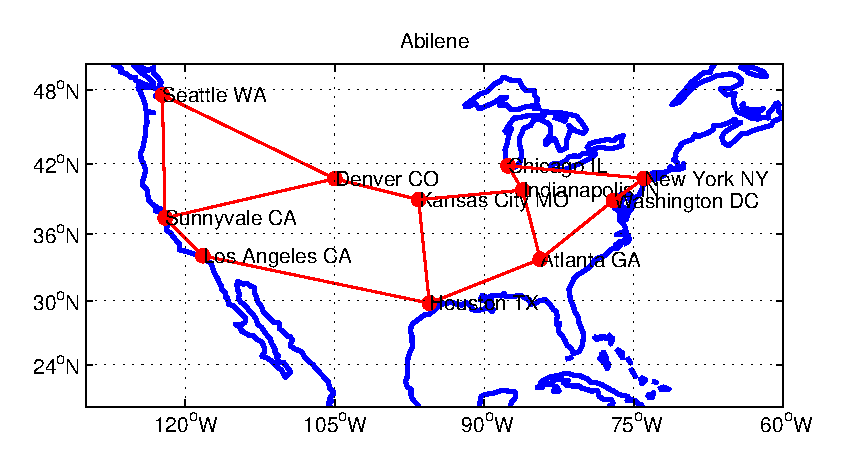
\includegraphics[width=\textwidth]{abilene_map.eps}
      \vspace{-5mm}
      \caption{Map of Abilene PoPs. \autoref{tab:traffic_matrix} is a
        router to router traffic matrix, but there is one router per
        PoP except in Atlanta, where there is a second router. The
        router numbers in the table are alphabetical.}
      \label{fig:abilene_2004_map}
    \end{subfigure}

    \vspace{3mm}
    \begin{subfigure}[b]{\oneup}
      \centering
      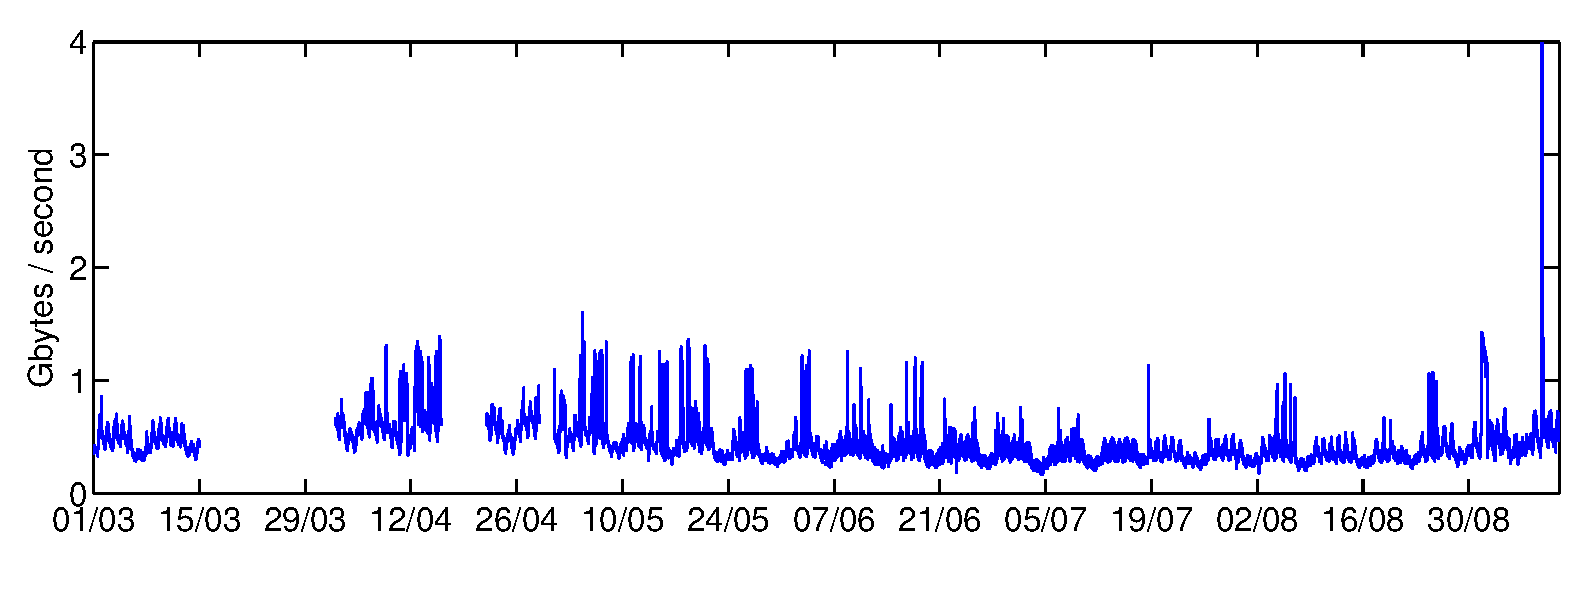
\includegraphics[width=\textwidth]{Abilene_2004_totals.eps}
      \vspace{-9mm}
      \caption{Abilene 5 minute totals of the traffic matrix from
        March 1st to September 11th, 2004.}
      \label{fig:abilene_2004_a}
    \end{subfigure}

    \vspace{3mm}
    \begin{subfigure}[b]{\oneup}
      \centering
      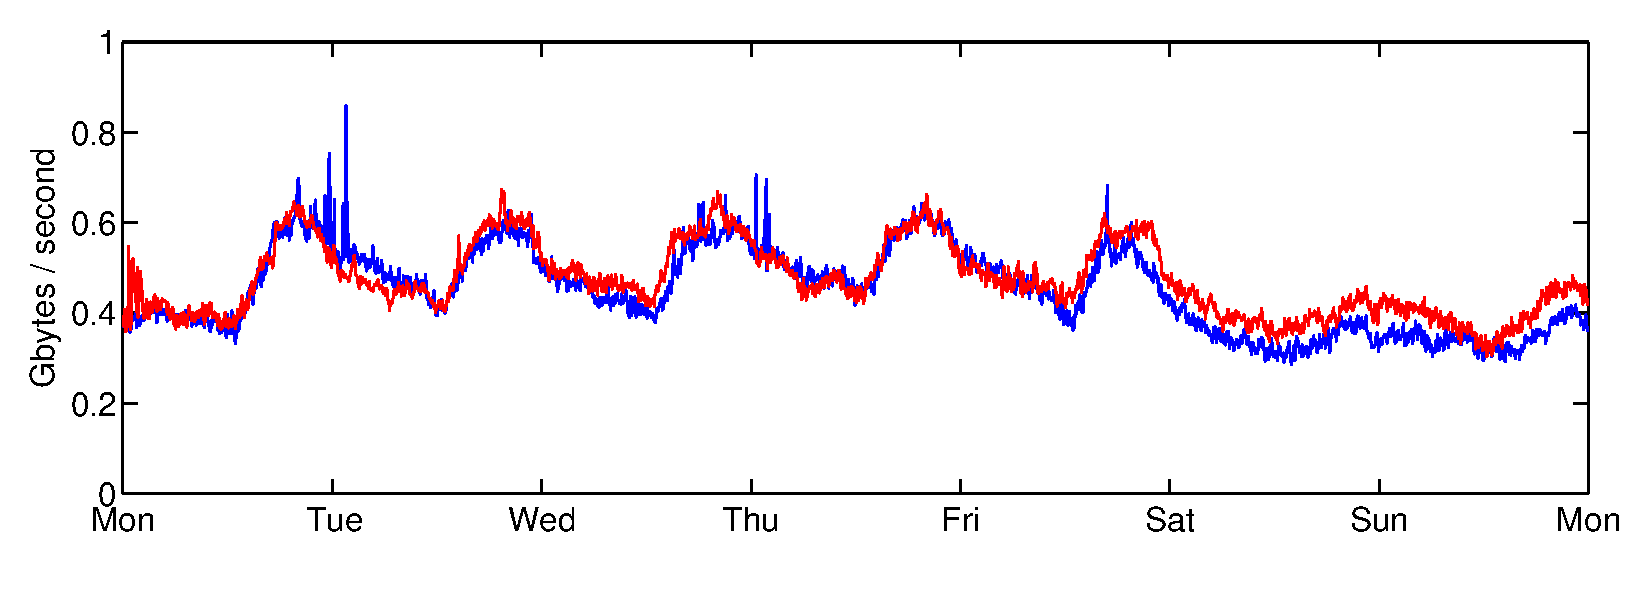
\includegraphics[width=\textwidth]{Abilene_2004_totals_short.eps}
      \vspace{-8mm}
      \caption{The weeks starting March 1st (blue), and March 8th (red).}
      \label{fig:abilene_2004_b} 
    \end{subfigure}  
       
    \vspace{2mm}
    \caption{Abilene, 2004\label{fig:abilene_2004}}
  \end{center}
\end{figure}         

We have endeavoured to put this data into an easily read format, and
placed it onto a web server at 
\url{http://www.maths.adelaide.edu.au/matthew.roughan/traffic_matrices.html},
where we will also place other TM datasets as far as possible, for
comparison studies, or as test datasets for education.

The data illustrates a number of properties of the data, perhaps most notably
the fact that many datasets have anomalous ``spikes'' (these are often
real, but may also be artefacts in the data), and periods of missing
data. The question of how these arise then naturally leads to our next
chapter on measuring traffic matrices. 
  